\documentclass[12pt,twoside]{book}
\usepackage{imakeidx}
\input{tex/header}
\input{tex/color_thm_head}

% Additional Packages and Libraries
\usepackage{wrapfig}
\usepackage{enumitem}
\usetikzlibrary{shapes}
\usetikzlibrary{decorations.pathmorphing,decorations.pathreplacing,decorations.shapes,decorations.text}
\makeindex[columns=3,intoc,columnseprule]
\tikzset{
    GRU/.pic={
        \draw[accent,line width=7,opacity=0.5,decorate,decoration={random steps},rounded corners] (-3,0.25) -- (3,0.25);
        \node[anchor=south] (sf) at (-2,0) {
\includegraphics[height=3cm]{images/stickfigure.png}};
        \node[anchor=south] at (0,0) {
\includegraphics[width=6cm,height=0.5cm]{images/grass.png}};
        \node[anchor=north] at (2,6) {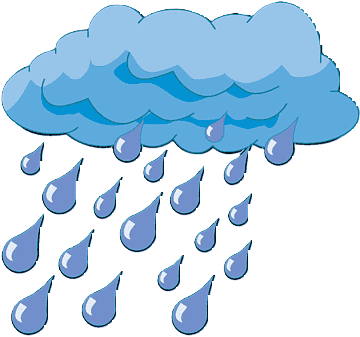
\includegraphics[height=3cm]{images/rain.png}};
        \node[anchor=south] at (sf.east) {
\includegraphics[height=2.5cm]{images/Umbrella-3-Clip-Art.png}};
    }
}

\tikzset{
    GR/.pic={
        \draw[accent,line width=7,opacity=0.5,decorate,decoration={random steps},rounded corners] (-3,0.25) -- (3,0.25);
        \node[anchor=south] (sf) at (-2,0) {
\includegraphics[height=3cm]{images/stickfigure.png}};
        \node[anchor=south] at (0,0) {
\includegraphics[width=6cm,height=0.5cm]{images/grass.png}};
        \node[anchor=north] at (2,6) {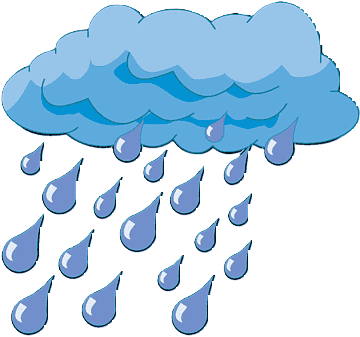
\includegraphics[height=3cm]{images/rain.png}};
    }
}

\tikzset{
    GU/.pic={
        \draw[accent,line width=7,opacity=0.5,decorate,decoration={random steps},rounded corners] (-3,0.25) -- (3,0.25);
        \node[anchor=south] (sf) at (-2,0) {
\includegraphics[height=3cm]{images/stickfigure.png}};
        \node[anchor=south] at (0,0) {
\includegraphics[width=6cm,height=0.5cm]{images/grass.png}};
        \node[anchor=south] at (sf.east) {
\includegraphics[height=2.5cm]{images/Umbrella-3-Clip-Art.png}};
    }
}

\tikzset{
    RU/.pic={
        \node[anchor=south] (sf) at (-2,0) {
\includegraphics[height=3cm]{images/stickfigure.png}};
        \node[anchor=south] at (0,0) {
\includegraphics[width=6cm,height=0.5cm]{images/grass.png}};
        \node[anchor=north] at (2,6) {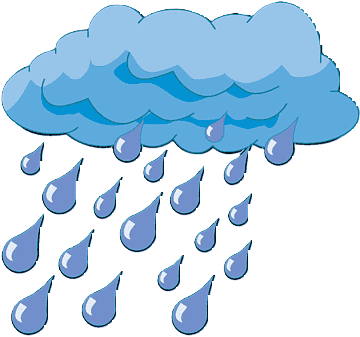
\includegraphics[height=3cm]{images/rain.png}};
        \node[anchor=south] at (sf.east) {
\includegraphics[height=2.5cm]{images/Umbrella-3-Clip-Art.png}};
    }
}

\tikzset{
    G/.pic={
        \draw[accent,line width=7,opacity=0.5,decorate,decoration={random steps},rounded corners] (-3,0.25) -- (3,0.25);
        \node[anchor=south] (sf) at (-2,0) {
\includegraphics[height=3cm]{images/stickfigure.png}};
        \node[anchor=south] at (0,0) {
\includegraphics[width=6cm,height=0.5cm]{images/grass.png}};
    }
}

\tikzset{
    R/.pic={
        \node[anchor=south] (sf) at (-2,0) {
\includegraphics[height=3cm]{images/stickfigure.png}};
        \node[anchor=south] at (0,0) {
\includegraphics[width=6cm,height=0.5cm]{images/grass.png}};
        \node[anchor=north] at (2,6) {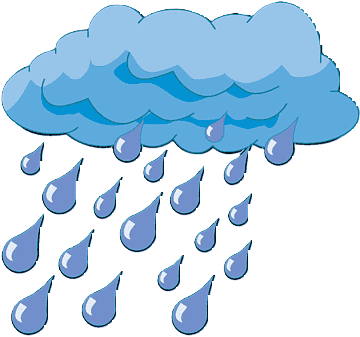
\includegraphics[height=3cm]{images/rain.png}};
    }
}

\tikzset{
    U/.pic={
        \node[anchor=south] (sf) at (-2,0) {
\includegraphics[height=3cm]{images/stickfigure.png}};
        \node[anchor=south] at (0,0) {
\includegraphics[width=6cm,height=0.5cm]{images/grass.png}};
        \node[anchor=south] at (sf.east) {
\includegraphics[height=2.5cm]{images/Umbrella-3-Clip-Art.png}};
    }
}

\tikzset{
    None/.pic={
        \node[anchor=south] (sf) at (-2,0) {
\includegraphics[height=3cm]{images/stickfigure.png}};
        \node[anchor=south] at (0,0) {
\includegraphics[width=6cm,height=0.5cm]{images/grass.png}};
    }
}

\tikzset{
    PlaneU/.pic={
        \node[anchor=south] (sf) at (-2,0) {
\includegraphics[height=3cm]{images/stickfigure.png}};
        \node[anchor=south] at (0,0) {
\includegraphics[width=6cm,height=0.5cm]{images/grass.png}};
        \node[anchor=south] at (sf.east) {
\includegraphics[height=2.5cm]{images/Umbrella-3-Clip-Art.png}};
        \node[xscale=-1,rotate=-30] at (2,4.5) {
\includegraphics[width=3cm]{images/zombie_girl_plane.png}};
    }
}

\tikzset{
    Plane/.pic={
        \node[anchor=south] (sf) at (-2,0) {
\includegraphics[height=3cm]{images/stickfigure.png}};
        \node[anchor=south] at (0,0) {
\includegraphics[width=6cm,height=0.5cm]{images/grass.png}};
        \node[xscale=-1,rotate=-30] at (2,4.5) {
\includegraphics[width=3cm]{images/zombie_girl_plane.png}};
    }
}

% Externalization Commands and Packages
\usetikzlibrary{external}
\tikzexternalize[prefix=tikz/]
% input command code based on 
% https://tex.stackexchange.com/questions/482557/how-to-externalize-tikz-pictures
% modified so that the tikz files are in the tikz folder where the exertanlized
% pictures are kept.
\newcommand{\inputtikz}[1]{%
  \tikzsetnextfilename{#1}%
  \input{tikz/#1.tikz}%
}

% Page Formattiing
\geometry{inner=1in,outer=0.5in,top=1in,bottom=0.75in}
\renewcommand{\chaptermark}[1]{ \markboth{#1}{} }
\renewcommand{\sectionmark}[1]{ \markright{#1}{} }

% New Commands

\newcommand{\answerbox}[1][1in]{
    % \begin{tcolorbox}[colframe=tertiaryaccent,colback=white,height=20pt,hbox,on line]
    %     \phantom{#1}
    % \end{tcolorbox}
    \phantom{\rule{0pt}{20pt}}\rule{#1}{0.2pt}
}

% Other Document Information

    \title{Foundational Discrete Math Notes}
    \author{Charles Rocca}
    % \date{2-10-2020}



\begin{document}

\maketitle


\tableofcontents
\listoffigures
\listoftables

\chapter{Symbolic Logic and Predicates}
    \section{Logical Statements}
    \begin{defn}[Statements]
    A \emph{statement}\index{statement} (or \emph{proposition}\index{proposition}) is a sentence which is true or false but not both.
\end{defn}
\begin{defn}[New Statements From Old]
    Given statements \(P\) and \(Q\):
    \begin{itemize}
        \item The \emph{negation}\index{negation} of a statement, \(\sim P\) or \(not\ P\), always has the opposite truth value.
        \item The \emph{conjunction}\index{conjunction} of two statements, \(P\wedge Q\) or \(P\ and\ Q\), is true when both statements are true.
        \item The \emph{disjunction}\index{disjunction} of two statements, \(P\vee Q\) or \(P\ or\ Q\), is true when either statement is true.
        % \item A \emph{conditional statement} with two statements, \(P\rightarrow Q\) or \(if\ P\ then \ Q\), is false when \(P\) is true and \(Q\) is false, it is otherwise true.
    \end{itemize}
\end{defn}


\begin{practiceprob}[Statements and Their Negations]\label{rainstatements}
    Fill in the negation for the statements: \(R\equiv\) ``It is raining.''; \(G\equiv\) ``The grass is wet.''; and \(U\equiv\) ``I have an umbrella.''
        \begin{itemize}
            \item \(\sim R\equiv\) \vspace{\baselineskip}
            \item \(\sim G\equiv\) \vspace{\baselineskip}
            \item \(\sim U\equiv\) \vspace{\baselineskip}
        \end{itemize}
\end{practiceprob}

\clearpage

\newcounter{n}
\setcounter{n}{1}
\begin{practiceprob}[Visualizing Truth Values]\label{mainimages}
    For each picture indicate all the statements from practice problem \ref{rainstatements} that apply to it by writing the appropriate letter or its negation.
    \begin{center}
        % \inputtikz{grass_zombies}
        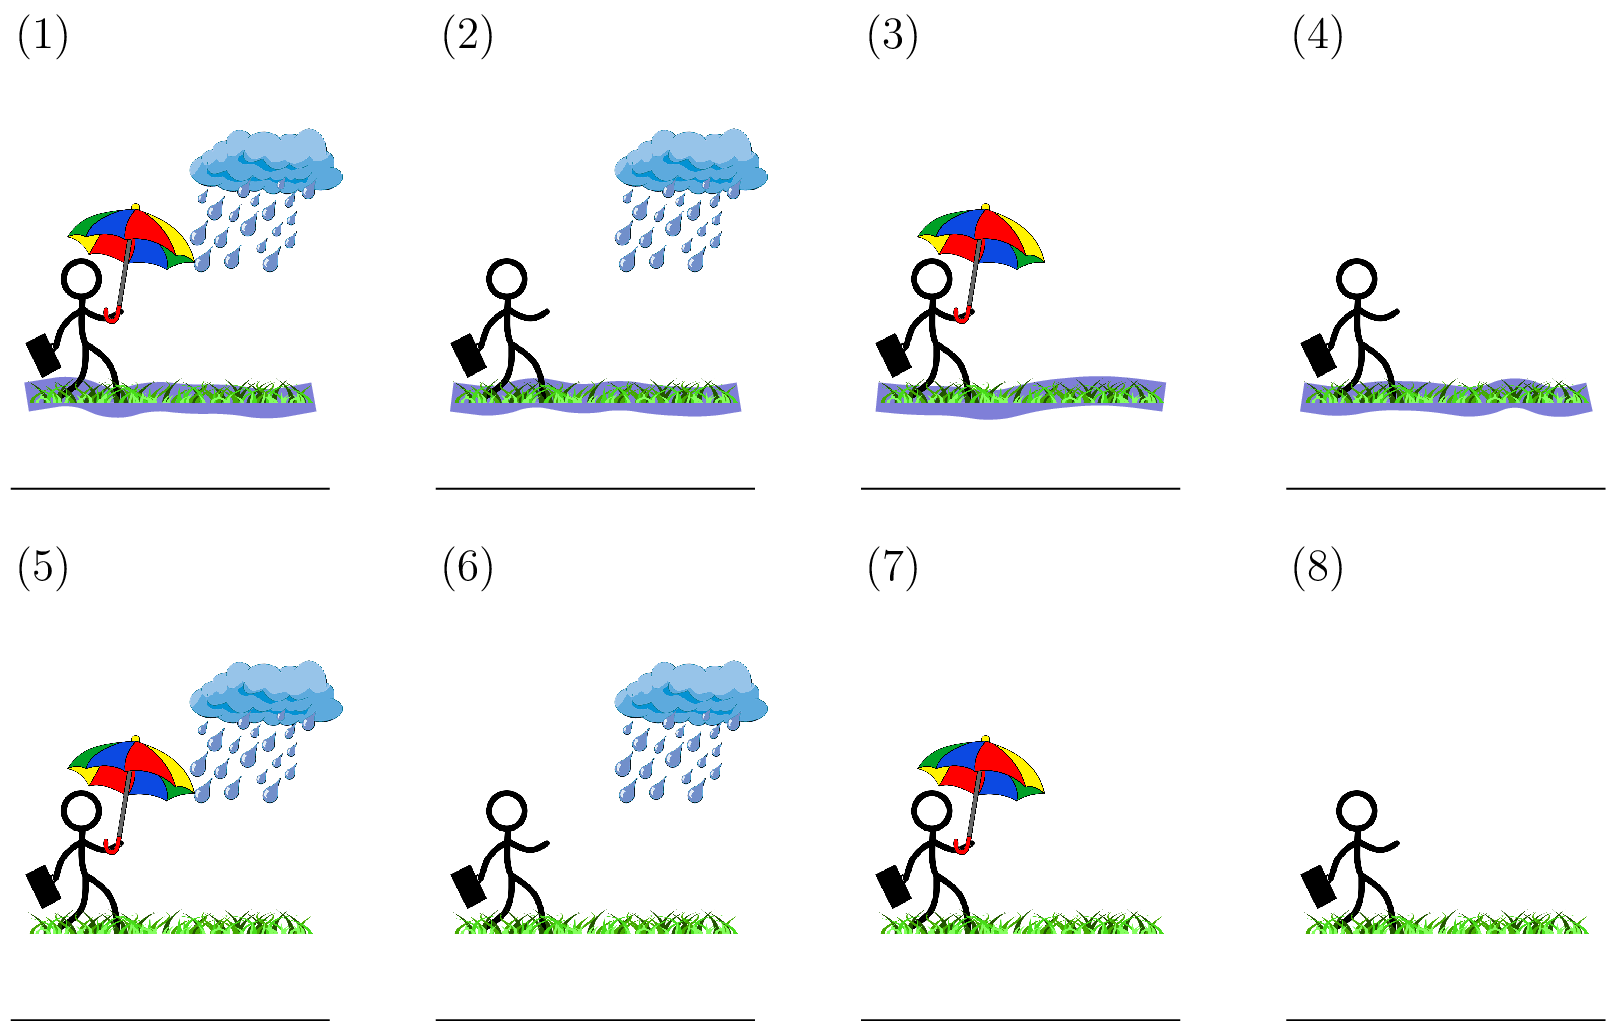
\includegraphics[scale=0.24,alt={Eight images with different configurations of a stick figure with out without rain or an umbrella or wet grass.},width=0.85\linewidth]{images/created/grass_zombies.png}
    \end{center}
\end{practiceprob}



\begin{practiceprob}[Relating Statements to Sets]
    For each region of the Venn Diagram, write down which picture from practice problem \ref{mainimages} belongs in that region.
    \begin{center}
        % \inputtikz{venn_zombies}
        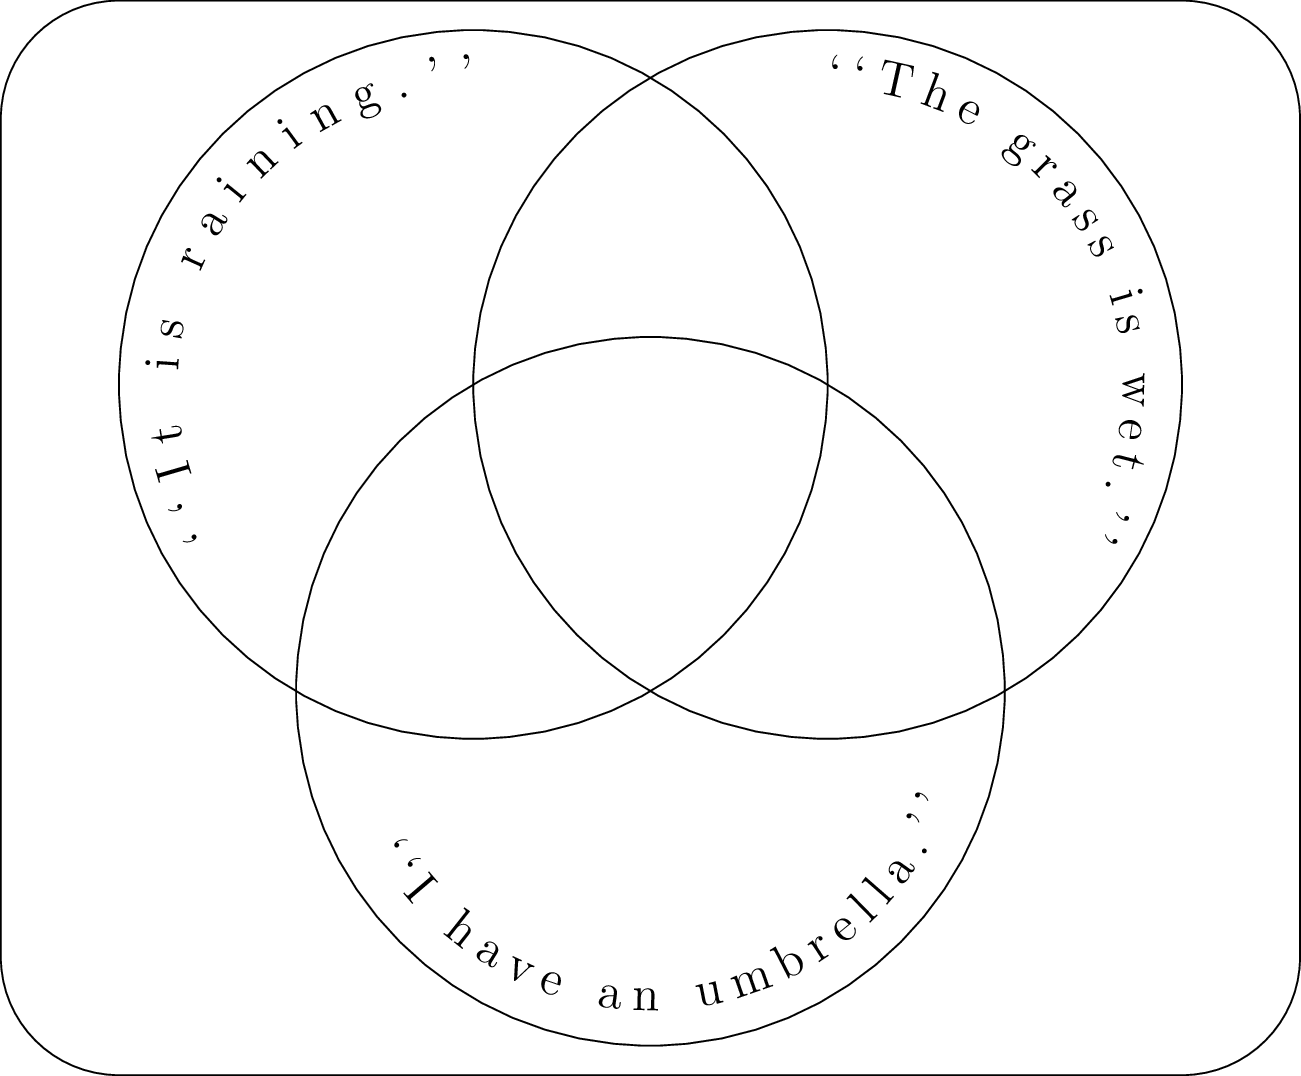
\includegraphics[scale=0.24,alt={Blank Venn diagram for organizing the previous images into three overlapping sets.},width=0.65\linewidth]{images/created/venn_zombies.png}        
    \end{center}    
\end{practiceprob}

\clearpage

\begin{practiceprob}[Combinations and Modifications of Statements]
    For each combination of statements, indicate which set of pictures from practice problem \ref{mainimages} make the statement true.
    \begin{multicols}{2}
    \begin{enumerate}
    \setlength{\itemsep}{10pt}
        \item \(U\wedge G\): 
        \item \(\sim(U\wedge G)\): 
        \item \(\sim U\wedge \sim G\): 
        \item \(U\vee G\): 
        \item \(\sim(U\vee G)\): 
        \item \(\sim U \vee \sim G\): 
    \end{enumerate}   
    \end{multicols}
\end{practiceprob}

\begin{practiceprob}[Negating Compound Statements]
    \setlength{\extrarowheight}{10pt}
    Using \(U\equiv\) ``I have an umbrella.'' and \(G\equiv\) ``The grass is wet.'' fill in the \emph{truth table} below.  You can refer to the previous practice problems and the images above to help you.
    \begin{center}
    \begin{tabular}{*{4}{c}*{5}{>{\centering}m{0.125\textwidth}}}
        \(U\) & \(G\) & \(\sim U\) & \(\sim G\) & \(U\wedge G\) & \(U\vee G\) & \(\sim (U\wedge G)\) & \(\sim (U\vee G)\) & \(U \wedge \sim G\) \tabularnewline\hline
        \(T\)&\(T\)&&&&&&&\tabularnewline\hline
        \(T\)&\(F\)&&&&&&&\tabularnewline\hline
        \(F\)&\(T\)&&&&&&&\tabularnewline\hline
        \(F\)&\(F\)&&&&&&&\tabularnewline\hline        
    \end{tabular}
    \end{center}
\end{practiceprob}



\begin{defn}[Tautology and Contradiction]
    A \emph{tautology}\index{tautology} is a statement that is always true and a \emph{contradiction}\index{contradiction} is a statement that is always false.  For example, in the figures in practice problem \ref{mainimages}, ``the grass is green'' is a tautology since it is always true, ``there is a zombie'' is a contradiction since it is always false.
\end{defn}

\begin{practiceprob}[True or False]
    For which pictures in practice problem \ref{mainimages} are the following sentences true?
    \begin{enumerate}
    \setlength{\itemsep}{10pt}
        \item ``The grass is green.'' 
        \item ``There is a zombie.'' 
        \item ``The grass is green'' \(\vee\) ``I have an umbrella.'' 
        % \item ``The grass is green'' \(\wedge\) ``I have an umbrella.'' 
        % \item ``There is a zombie'' \(\vee\) ``I have an umbrella.'' 
        \item ``There is a zombie'' \(\wedge\) ``I have an umbrella.'' 
        \item ``There is a zombie'' \(\vee\) ``the grass is green.'' 
        \item ``There is a zombie'' \(\wedge\) ``the grass is green.'' 
    \end{enumerate}    
\end{practiceprob}

\begin{exposition}{Some ``Basic'' Logical Rules}
So far we have identified the following ways to put together statements using \(\wedge\), \(\vee\), and \(\sim\):
\begin{itemize}
    \setlength{\itemsep}{25pt}
    \begin{multicols}{2}
        \item \emph{Negation (not)}\index{negation}: \(\sim P\)
        \item \emph{Conjunction (and)}\index{conjunction}: \(P\wedge Q\)
        \item \emph{Disjunction (or)}\index{disjunction}: \(P \vee Q\)
        \item \emph{Exclusive Or (xor)}\index{exclusive or}\index{exclusive or!xor}:\newline \(P \oplus Q \equiv (P\vee Q) \wedge \sim(P\wedge Q)\)
        \item \emph{Double Negation}\index{double negation}: \(\sim(\sim P)\equiv P\)
        \item \emph{DeMorgan's Laws}\index{Demorgan's Laws}: 
        \begin{itemize}
            \item \(\sim(P\wedge Q)\equiv \sim P \vee \sim Q\)
            \item \(\sim(P\vee Q)\equiv \sim P \wedge \sim Q\)
        \end{itemize}
        \item \emph{Commutative Law}\index{commutative law}: 
        \begin{itemize}
            \item \(P\vee Q\equiv Q \vee P\)
            \item \(P\wedge Q\equiv Q \wedge P\)
        \end{itemize}
\columnbreak
        \item \emph{Distributive Law}\index{distributive law}: 
        \begin{itemize}
            \item \(P\wedge (Q\vee R)\equiv P\wedge Q \vee P\wedge R\)
            \item \(P\vee (Q\wedge R)\equiv P\vee Q \wedge P\vee R\)
        \end{itemize}
        \item \emph{Associative Law}\index{associative law}: 
        \begin{itemize}
            \item \(P\wedge (Q\wedge R)\equiv (P\wedge Q) \wedge R\)
            \item \(P\vee (Q\vee R)\equiv (P\vee Q) \vee R\)
        \end{itemize}
        \item \emph{Identity Laws}\index{identity laws}:
        \begin{itemize}
            \item \(t \wedge P \equiv P\)
            \item \(c \vee P \equiv P\)
        \end{itemize}
        \item \emph{Inverse Laws}\index{inverse laws}:
        \begin{itemize}
            \item \(P \vee \sim P \equiv t\)
            \item \(P \wedge \sim P \equiv c\)
        \end{itemize}
        \item \emph{Domination Laws}\index{domination laws}:
        \begin{itemize}
            \item \(t \vee P \equiv t\)
            \item \(c \wedge P \equiv c\)
        \end{itemize}
    \end{multicols}
\end{itemize}
\index{laws!double negation}
\index{laws!DeMorgan's}
\index{laws!commutative}
\index{laws!distributive}
\index{laws!associative}
\index{laws!identity}
\index{laws!inverse}
\index{laws!domination}
\end{exposition}
\clearpage

\section{Implications}
    

\begin{defn}[Implications/Conditional Statements]
    A \emph{conditional statement}, or {\em implication}, is a compound statement of the form {\em ``if \(P\), then \(Q\).''}  The first statement, \(P\), is called the {\em hypothesis} or {\em premise} and the second is the {\em conclusion}.  Conditionals can also be read {\em ``\(P\) implies \(Q\),''} {\em ``\(P\) only if \(Q\),''}, {\em ``\(Q\), if \(P\).''}  Notationally, we write ``if \(P\), then \(Q\)'' as \(P\rightarrow Q\).
\end{defn}

\setcounter{n}{1}
\begin{practice}[label=GRimages]{When are Implications False}
\setlength{\extrarowheight}{10pt}
    Looking at the following images, 
    \begin{center}
        \begin{tikzpicture}
            \foreach \p/\x in {GR/0,G/4,R/8,None/12}{
                \pic[scale=0.5,transform shape] at (\x,0) {\p};
                \node at (\x-1,2.5) {(\then)};
                \stepcounter{n};
            }
        \end{tikzpicture}
    \end{center}
    for which images is the statement 
        \begin{center}\emph{``If it is raining, then the grass is wet'' (\(R\rightarrow G\))}\end{center}
    false?\vspace{\baselineskip}\newline\hspace*{0pt}\hrulefill\vspace{\baselineskip}\newline
    Why is it false in those cases?\hrulefill\vspace{0.75\baselineskip}\newline  
    \hspace*{0pt}\hrulefill\vspace{\baselineskip}\newline
    In what situations must it then be true?\hrulefill\vspace{\baselineskip}\newline
    \hspace*{0pt}\hrulefill\vspace{\baselineskip}\newline
    Use the same sort of reasoning to try and fill in the following \emph{truth table}\index{truth table}.
    \begin{center}
    \begin{tabular}{*{4}{|c}*{5}{|>{\centering}m{0.125\textwidth}}|}\hline
        \(R\) & \(G\) & \(\sim R\) & \(\sim G\) & \(R\rightarrow G\) & \(G\rightarrow R\) & \(\sim R\rightarrow \sim G\) & \(\sim G\rightarrow \sim R\) & \(R\wedge \sim G\) \tabularnewline\hline
        &&&&&&&&\tabularnewline\hline
        &&&&&&&&\tabularnewline\hline
        &&&&&&&&\tabularnewline\hline
        &&&&&&&&\tabularnewline\hline        
    \end{tabular}
    \end{center}
\end{practice}

\clearpage

\begin{practice}{True or False: The Return}
    In practice problem \ref{GRimages} for which images are these true?
    \begin{enumerate}
    \setlength{\itemsep}{10pt}
        \item If ``there is a zombie,'' then ``the grass is wet.'' \hrulefill
        \item If ``there is a zombie,'' then ``it is raining.'' \hrulefill
        \item If ``it is raining,'' then ``the grass is green.'' \hrulefill
        \item If ``the grass is wet,'' then ``the grass is green.'' \hrulefill
    \end{enumerate}
\end{practice}



\begin{expository}{Conditionals and Their Relations}
    Starting with a conditional \(P \rightarrow Q\) we can write the following:
    \begin{multicols}{2}
        \begin{enumerate}
            \item \emph{Converse}\index{converse}: \(Q\rightarrow P\)
            \item \emph{Inverse}\index{inverse}: \(\sim P\rightarrow \sim Q\)
            \item \emph{Contrapositive}\index{contrapositive}: \(\sim Q\rightarrow \sim P\)
            \item \emph{Negation}\index{negation}: \(P\wedge \sim Q\)
        \end{enumerate}
    \end{multicols}
    Where \((P\rightarrow Q) \equiv (\sim Q \rightarrow \sim P)\), 
    \((Q\rightarrow P) \equiv (\sim P \rightarrow \sim Q)\), 
    and \(\sim (P\rightarrow Q) \equiv (P \wedge \sim Q)\).
    
    Further we can say \(P\rightarrow t\) and \(c\rightarrow Q\) are \emph{vacuously true}\index{vacuously true} because their negations are always false:
        \[\sim (P\rightarrow t) \equiv (P \wedge c) \equiv c\]
    and
        \[\sim (c\rightarrow Q) \equiv (c \wedge \sim Q) \equiv c.\]
\end{expository}

\setcounter{n}{1}
\begin{practice}{Making Arguments}
    If we assume it is true that ``If I carry an umbrella, then zombies dive bomb me,'' then which pictures should we look at? \answerbox
    \begin{center}
        \begin{tikzpicture}
            \foreach \p/\x in {PlaneU/0,U/4,Plane/8,None/12}{
                \pic[scale=0.5,transform shape] at (\x,0) {\p};
                \node at (\x-1,2.5) {(\then)};
                \stepcounter{n};
            }
        \end{tikzpicture}
    \end{center}
    What if we also assume that it is true that ``I am carrying an umbrella,''
    which picture(s) do we look at then \answerbox, are there zombies dive bombing me \answerbox?\vspace{\baselineskip}

    \noindent%
    What if we also assume that it is true that ``zombies dive bomb me,'' which picture(s) do we look at then \answerbox, am I carrying an umbrella \answerbox?
    
\end{practice}

\clearpage

\begin{expository}{More Rules and Arguments}
    Given statements \(P\) and \(Q\) the following are some common valid and invalid argument forms.
    \vspace{\baselineskip}

    \begin{tabular}{*{4}{p{0.22\textwidth}}}
    \emph{Modus Ponens}\index{modus ponens}:
        \[
            \begin{array}{ll}
                P\rightarrow Q  \\
                P \\\hline
                \therefore\ Q
            \end{array}
        \] &
    \emph{Modus Tollens}\index{modus tollens}:
        \[
            \begin{array}{ll}
                P\rightarrow Q  \\
                \sim Q \\\hline
                \therefore\ \sim P
            \end{array}
        \] &
    \emph{Converse Error}\index{converse error}:
        \[
            \begin{array}{ll}
                P\rightarrow Q  \\
                Q \\\hline
                \therefore\ P
            \end{array}
        \] &
    \emph{Inverse Error}\index{inverse error}:
        \[
            \begin{array}{ll}
                P\rightarrow Q  \\
                \sim P \\\hline
                \therefore\ \sim Q
            \end{array}
        \] \tabularnewline
    \emph{Disjunctive\newline Syllogism}\index{disjunctive syllogism}:
        \[
            \begin{array}{ll}
                P\vee Q  \\
                \sim P \\\hline
                \therefore\ Q
            \end{array}
        \] &
    \emph{Law of\newline Simplification}\index{law of simplification}:
        \[
            \begin{array}{ll}
                P\wedge Q  \\ \hline
                \therefore\ P\ \text{and}\ Q
            \end{array}
        \] &
    \emph{Transitivity}\index{transitivity}:
        \[
            \begin{array}{ll}
                P\rightarrow Q  \\
                Q\rightarrow R \\\hline
                \therefore\ P\rightarrow R
            \end{array}
        \] &
    \emph{Contradiction}\index{contradiction}:
        \[
            \begin{array}{ll}
                P \wedge \sim Q\rightarrow c  \\\hline
                \therefore\ P\rightarrow Q
            \end{array}
        \] 
    \end{tabular}
\end{expository}
\clearpage

\section{Using Logical Laws and Arguments}
    Add a section with examples of simplifying or writing ``proofs'' with logical laws and stuff.
\clearpage

\section{Predicates}
    \begin{defn}[Predicates]
    A \emph{predicate}\index{predicate} is a statement containing a finite number of variables. The predicate becomes true or false based on the value of the variables.
\end{defn}
\begin{exposition}[Sample Predicates]
Find values for the variables which make the predicates true or false.
\begin{sides}
    \begin{itemize}
    \setlength{\itemsep}{18pt}
        \item \(P(x): x\in\bbZ \wedge x>5\)
        \item \(Q(x): x\in\bbR \wedge x>5\)
        \item \(G(a,b):  a>b\)
        \item \(\forall a,b\in\bbZ: G(a,b) \rightarrow G(a^3,b^3)\)
        \item \(S(n,m): n^2>m\)
    \end{itemize}
\tcblower
    \begin{itemize}
    \setlength{\itemsep}{18pt}
        \item \(\exists n\in\bbZ: S(n,25)\)
        \item \(\forall n\in\bbZ: S(n,0)\)
        \item \(\exists n\in\bbZ: \sim S(n,0)\)
        \item \(\forall a,b\in R: G(a,b)\leftrightarrow S(a,b)\)
        \item \(\forall n\in\bbN\ \exists a,b,c\in\bbZ: a^n+b^n=c^n\)
    \end{itemize}
\end{sides}    
\end{exposition}

\begin{practiceprob}[Shapes, Colors, and Zombies, Oh My!!]
Use figure \ref{fig:Tarski} on page \pageref{fig:Tarski} to identify when these predicates are true or false.
\begin{sides}
    \begin{itemize}
    \setlength{\itemsep}{18pt}
        \item \(C(x):\) \(x\) is a consonant
        \item \(V(x):\) \(x\) is a vowel
        \item \(Z(x):\) \(x\) is a zombie
        \item \(S(x):\) \(x\) is a stick figure
        \item \(N(x):\) \(x\) is a brain
        \item \(R(x):\) \(x\) is \textcolor{red!60!black}{\bfseries\em red}
    \end{itemize}
    \tcblower
    \begin{itemize}
    \setlength{\itemsep}{18pt}
        \item \(B(x):\) \(x\) is \textcolor{blue!50!black}{\em\bfseries blue}
        \item \(G(x):\) \(x\) is \textcolor{green!60!black}{\bfseries\em green}
        \item \(P(x):\) \(x\) is a pentagon (5-sides)
        \item \(H(x):\) \(x\) is a heptagon (7-sides)
        \item \(W(x,y):\) \(x\) is in the same row as \(y\)
        \item \(L(x,y):\) \(x\) is in the same column as \(y\)
    \end{itemize}
\end{sides}
\end{practiceprob}

\clearpage

\begin{figure}[H]
    \centering
    % \inputtikz{tarski_world}
    \includegraphics[scale=0.06,alt={Ten by ten grid with various shapes letters and figures},width=0.9\linewidth]{images/created/tarski_world.png}
    \caption{Tarski's World}
    \label{fig:Tarski}
\end{figure}

\clearpage

\begin{exposition}[Truth Sets]

Given a predicate, the \emph{truth set}\index{truth set} for that predicate is the collection of all elements where it is true.  For example for \(V(x): x\ \text{is a vowel}\), the truth set is 
    \[T_V=\left\{a,e,i,o,u,y\right\}\] and for \(P(x): x\ \text{is a pentagon}\) the truth set is \[T_P=\left\{t,a,u,h,k,o,p\right\}.\] 
Figure \ref{fig:VP_Venn} shows how these two sets are related, in particular we can see that 
    \[V(x)\wedge P(x)\ \text{and}\ V(x)\wedge \sim P(x)\ \text{and}\ \sim V(x)\wedge P(x)\]
are all true if we pick the right value of \(x\).

\begin{figure}[H]
    \centering
    % \inputtikz{truth_set_venn}
    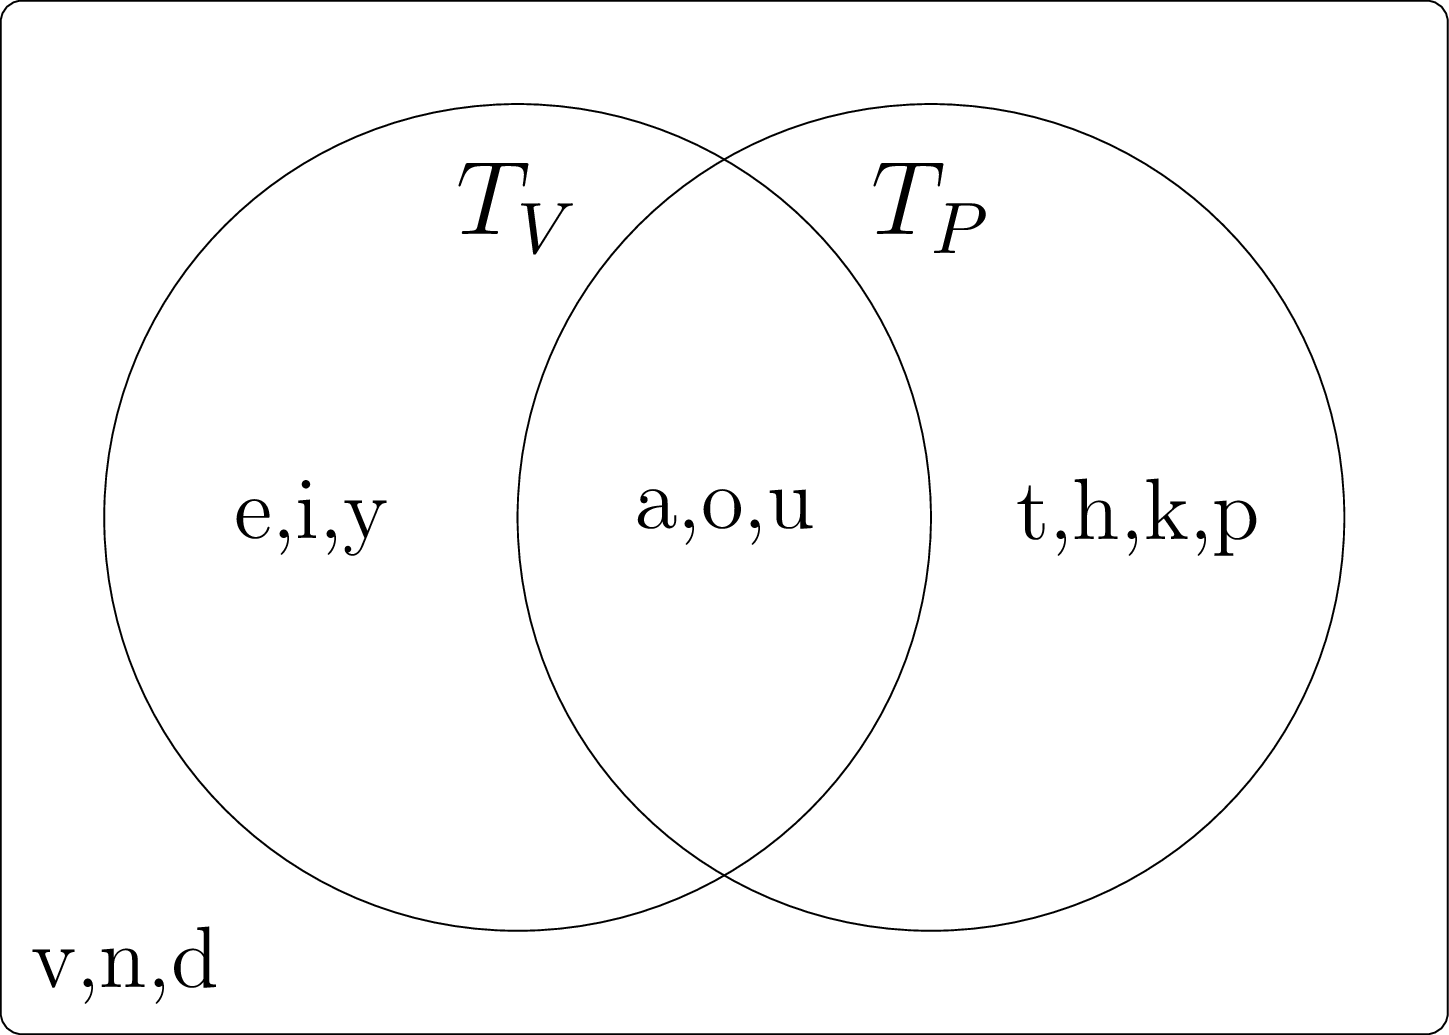
\includegraphics[scale=0.06,alt={Venn diagram of two truth sets},width=0.75\linewidth]{images/created/truth_set_venn.png}
    \caption{Venn Diagram of \(T_V\) and \(T_P\)}
    \label{fig:VP_Venn}
\end{figure}





\noindent
The predicates like \[W(x,y):\, x\ \text{is in the same row as}\ y\]
would have the truth set
\[T_W=\left\{(e,h),(h,e),(u,p),(p,u),(i,k),(k,i),(a,d),(d,a),(t,o),(o,t)\right\}.\]
\end{exposition}

\clearpage

\begin{practiceprob}[Truth Zombies]
Using figure \ref{fig:Tarski}, fill in the \emph{truth set} for each of the predicates.
\begin{enumerate}
    \item The truth set for \(G(x)\) is \[T_G=\left\{\phantom{\rule{0.8\textwidth}{20pt}}\right\}\]
    \item The truth set for \(H(x)\) is \[T_H=\left\{\phantom{\rule{0.8\textwidth}{20pt}}\right\}\]
    \item Fill in the Venn Diagram in figure \ref{fig:GH_Venn} for each of the previous truth sets.
    \item Where would the set \(T_Z\) fit in figure \ref{fig:GH_Venn}?  What does that tell us about the statement \[\forall x: Z(x)\rightarrow G(x)?\]
    \item The truth set for \(L(x,y)\) is \[ T_L=\left\{\phantom{\rule{0.8\textwidth}{20pt}}\right\}\]
\end{enumerate}
\begin{figure}[H]
    \centering
    % \inputtikz{empty_truth_venn}
    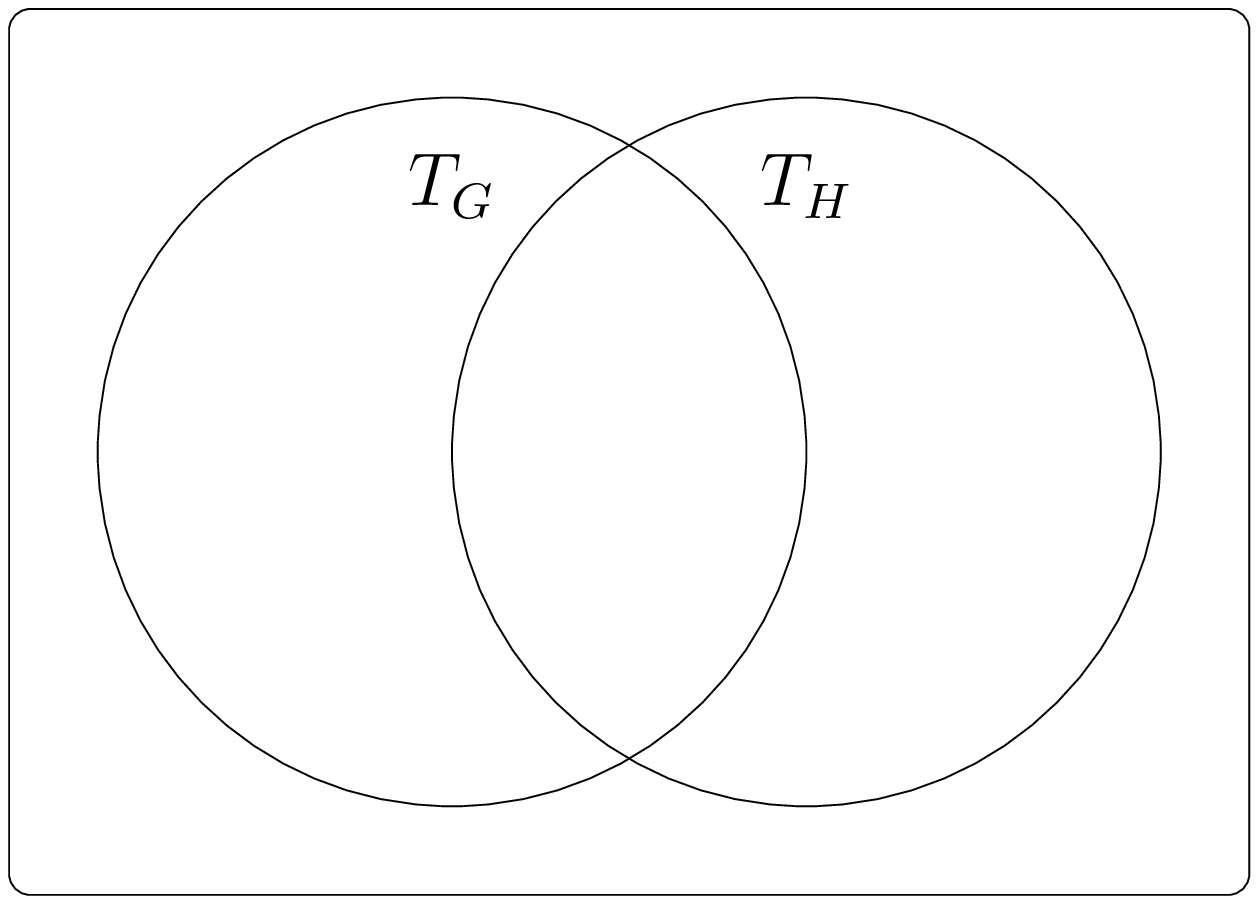
\includegraphics[scale=0.06,alt={Blank venn diagram for two truth sets},width=0.75\linewidth]{images/created/empty_truth_venn.png}
    \caption{Venn Diagram of \(T_G\) and \(T_H\)}
    \label{fig:GH_Venn}
\end{figure}
\end{practiceprob}

\clearpage

\begin{exposition}[Quantified Predicates]
% Examples
Recall \(\exists\) is the \emph{existential quantifier}\index{existential quantifier} and \(\forall\) the \emph{universal quantifier}\index{universal quantifier}.  Now, if we write 
    \[\exists x: V(x)\wedge P(x)\]
we can read that as 
\begin{center}
    \textit{``there exists a vowel which is also a pentagon''}
\end{center} 
or in plainer English 
\begin{center}
    \textit{``some vowels are pentagons.''}
\end{center} 
Is the previous statement true or false? How can we see it in the Venn Diagram in figure \ref{fig:VP_Venn}?\vspace{3\baselineskip}

\noindent
And, if we write 
    \[\forall x: V(x)\vee P(x)\]
we read it as 
\begin{center}
    \textit{``all the shapes are vowels or pentagons.''}
\end{center} Is this true or false? How can we see it in the Venn diagram in figure \ref{fig:VP_Venn}?\vspace{3\baselineskip}

\noindent
In addition to using them one at a time we can combine them like this 
    \[\forall x\,  \exists y: C(x)\rightarrow L(x,y)\] 
which we read as 
\begin{center}
    \textit{``every consonant shares a column with some letter,''}
\end{center} or like this \[\exists y\, \forall x: C(x)\rightarrow L(x,y)\] which we read as 
\begin{center}
    \textit{``some letter shares a column with every consonant.''}
\end{center} Which of the previous two statements is true and which is false?  How do we know?\vspace{3\baselineskip}
\end{exposition}

\clearpage

\begin{practiceprob}[Tarski's Zombies]
% Exercises
Referring to figure \ref{fig:Tarski}, which of the following predicates are true and which are false?  Try to write each in plain English and negate the false predicates.
\begin{enumerate}
\setlength{\itemsep}{40pt}
    \item \(\displaystyle\forall x: H(x)\rightarrow C(x)\)
    \item \(\displaystyle\exists x: V(x)\wedge R(x)\)
    \item \(\displaystyle\forall x\, \exists y: C(x)\rightarrow V(y)\wedge L(x,y)\)
    \item \(\displaystyle\forall x\, \forall y: C(x)\wedge V(y)\rightarrow L(x,y)\vee W(x,y)\)
    \item \(\displaystyle\forall x\in T_Z, \exists y\in T_N: W(x,y)\)
    \item \(\displaystyle\exists y\in T_N, \forall x\in T_Z: W(x,y)\)\vspace{35pt}
\end{enumerate}
Finally, look at figure \ref{fig:Tarski} and construct three quantified statements of your own using the given predicates.  Make two of them true and one a lie.  Make at least one of them doubly quantified.
\begin{itemize}
\setlength{\itemsep}{40pt}
    \item Truth:
    \item Truth:
    \item Lie:\vspace{35pt}
\end{itemize}
\end{practiceprob}



\cleardoublepage

\chapter{Sequences and Sums}

\chapter{Sets, Relations, and Functions}

\chapter{Combinatorics}

\chapter{Graphs and Trees}


\appendix

\chapter{Logic Reference Table}

\chapter{Sets Reference Table}

\printindex

\end{document}